\section{Våben og ammunition til jagt}

\begin{frame}
  \vspace{3em}
  \begin{center}
    {\LARGE \textbf{Bekendtgørelse om våben og ammunition der må anvendes til jagt m.v.}} \\
    \vspace{1em}
    BEK nr 1479 af 05/12/2023 \\ §§ 1-3
  \end{center}
\end{frame}

\begin{frame}{Tilladte skydevåben til jagt og regulering (§1)}
    \begin{itemize}
        \item \textbf{Glatløbede haglgeværer}:
          \begin{itemize}
            \item Pibelængde ≥ 55 cm
            \item Højst kaliber 12
            \item Højst 2 patroner (permanent begrænsning hvis konstrueret til mere)
          \end{itemize}
        \item \textbf{Riflede våben}:
          \begin{itemize}
            \item Manuelt repeterende
            \item Ikke helautomatiske/fuldautomatiske
            \item Halvautomatiske: Højst 3 patroner (permanent begrænsning hvis mere; max 2 i magasin + 1 i kammer)
            \item Luftgeværer: Min projektildiameter ≥ 5,5 mm
          \end{itemize}
        \item \textbf{Forbudt}: Revolvere og pistoler
    \end{itemize}
\end{frame}

\begin{frame}{Jagtammunition til riflede våben}
\framesubtitle{Tilladt ammunition til jagt og regulering af vildt}

\tiny
\begin{tabular}{|c|p{2.8cm}|c|c|c|c|c|}
\hline
\textbf{Klasse} & \textbf{Vildtart} &
\textbf{\begin{tabular}{@{}c@{}}Kuglediam.\\$\geq$6 mm\\$E_{100}\geq$2000 J\end{tabular}} &
\textbf{\begin{tabular}{@{}c@{}}Kuglediam.\\$\geq$5,5 mm\\$E_{100}\geq$800 J\end{tabular}} &
\textbf{\begin{tabular}{@{}c@{}}$E_{100}$\\$\geq$175 J\end{tabular}} &
\textbf{\begin{tabular}{@{}c@{}}$E_0$\\$\geq$150 J\end{tabular}} &
\textbf{\begin{tabular}{@{}c@{}}$V_0$\\$\geq$200\\m/sek.\textsuperscript{*}\end{tabular}} \\
\hline
1 & Kronvildt, Dåvildt, Sikavildt, Muflon, Vildsvin & $\times$ & & & & \\
\hline
2 & Råvildt, Sæler & $\times$ & $\times$ & & & \\
\hline
3 & Ræv, Vaskebjørn, Mårhund, Hare, Sumpbæver, Skarv, Gæs & $\times$ & $\times$ & $\times$ & & \\
\hline
4 & Husmår, Ilder, Mink, Vildkanin, Bisamrotte, Hønsefugle, Blishøne, Ænder, Måger & $\times$ & $\times$ & $\times$ & $\times$ & \\
\hline
5 & Duer, Kragefugle, Vadefugle, Stære & $\times$ & $\times$ & $\times$ & $\times$ & $\times$ \\
\hline
\end{tabular}

\vspace{0.3em}
\begin{footnotesize}
\textsuperscript{*} Luftdrevet: kuglediam.\ $\geq$ 5,5 mm \quad
\textsuperscript{1} Fx kal.\ .243, 6,5$\times$55, .270, .308, 30-06 \quad
\textsuperscript{2} Fx kal.\ 22-250, .222, .223 \\
\textsuperscript{3} Fx kal.\ .17 Rem, .22 Hornet, .221 Rem, .17 HMR \quad
\textsuperscript{4} Fx kal.\ .22 LR
\end{footnotesize}

\end{frame}

\begin{frame}{Begrænsninger for haglgeværer}
    \begin{itemize}
        \item Må bruges på vildt i \textbf{klasse 2–5} (jf. bilag 1) – ikke på sæler
        \item Råbuk med hagl: \textbf{Ikke} 16. maj – 15. juli
        \item Kaliber < 20: Kun klasse 5-vildt
        \item Permanente begrænsninger (plug/magasin-blokering) tillader brug af større magasiner
        \item \textbf{Generelt}: Våbnet skal være i forsvarlig stand
        \item \textbf{Ikke tilladt}: Helautomatiske rifler (undt. særlige tilladelser fra Naturstyrelsen ved vildtskader)
    \end{itemize}
\end{frame}

\begin{frame}{Krav til haglpatroner i glatløbede haglgeværer}
    \begin{itemize}
        \item \textbf{Vægtfylde og udgangshastighed (V1,5)}:
          \begin{itemize}
            \item ≥ 7 g/cm³: Ingen minimumshastighedskrav
            \item ≤ 9 g/cm³: Mindst 400 m/sek
            \item > 9 g/cm³: Mindst 375 m/sek
          \end{itemize}
        \item \textbf{Maks. hagl-diameter}: 4 mm
        \item \textbf{Forbudt}: Kuglepatroner i glatløbede haglgeværer
        \item \textbf{Blyhagl – totalforbud} (fra 202X):
          \begin{itemize}
            \item Må ikke forhandles, medtages eller anvendes til jagt/regulering
            \item Må ikke medtages eller anvendes til flugtskydning (inkl. skydebaner)
          \end{itemize}
    \end{itemize}
\end{frame}

\begin{frame}{Jagtammunition til riflede våben}
    \begin{itemize}
        \item \textbf{Generelt}: Må bruges til arter i bilag 1 – minimumskrav skal overholdes
        \item \textbf{Klasse 1 \& 2 vildt} (jf. bilag 1):
          \begin{itemize}
            \item Projektilet skal være \textbf{ekspanderende} eller \textbf{fragmenterende}
          \end{itemize}
        \item \textbf{Blyindhold} ≥ 1 vægtprocent:
          \begin{itemize}
            \item Forbudt at medtage eller anvende til jagt/regulering
          \end{itemize}
        \item \textbf{Undtagelser fra blyforbuddet}:
          \begin{itemize}
            \item Randtænding-ammunition
            \item Ammunition fra luft- og fjedervåben
          \end{itemize}
        \item \textbf{Totalforbud}: Våben/ammunition i kaliber \textbf{50 BMG}
        
    \end{itemize}
\end{frame}

\begin{frame}{Maksimale skudafstande}
    \begin{itemize}
        \item Råvildt (hagl str. 1-2) max 20m
        \item Gæs, ræv (hagl str. 2-3) max 25m
        \item Ænder, fasaner, hare, duer (hagl str. 2-5) max 30m
        \item Bekkasin, snepper, agerhøns (hagl str 5-7 (max 30m)
    \end{itemize}
\end{frame}

\begin{frame}{Kend dit gevær}
    \begin{center}
        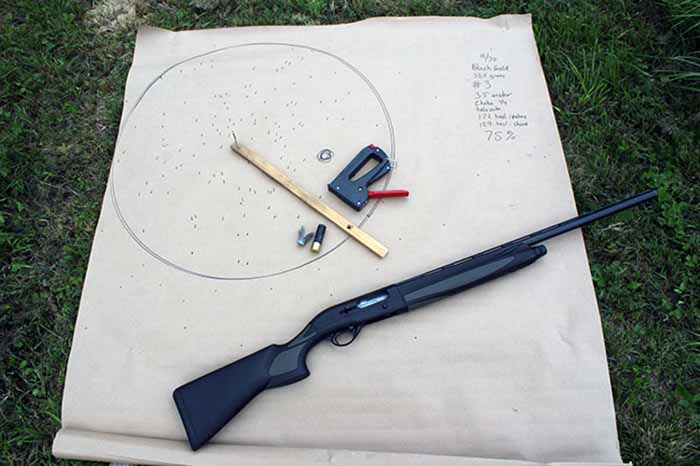
\includegraphics[width=0.7\textwidth]{Billeder/Andet/skudtest2.jpg}
        % Eller: [height=0.6\textheight] for højde-baseret skalering
    \end{center}
    
    % Her kan du tilføje tekst under billedet
    \vspace{1em}
    
\end{frame}




\begin{frame}{Jagtvåben typer}
    \begin{center}
        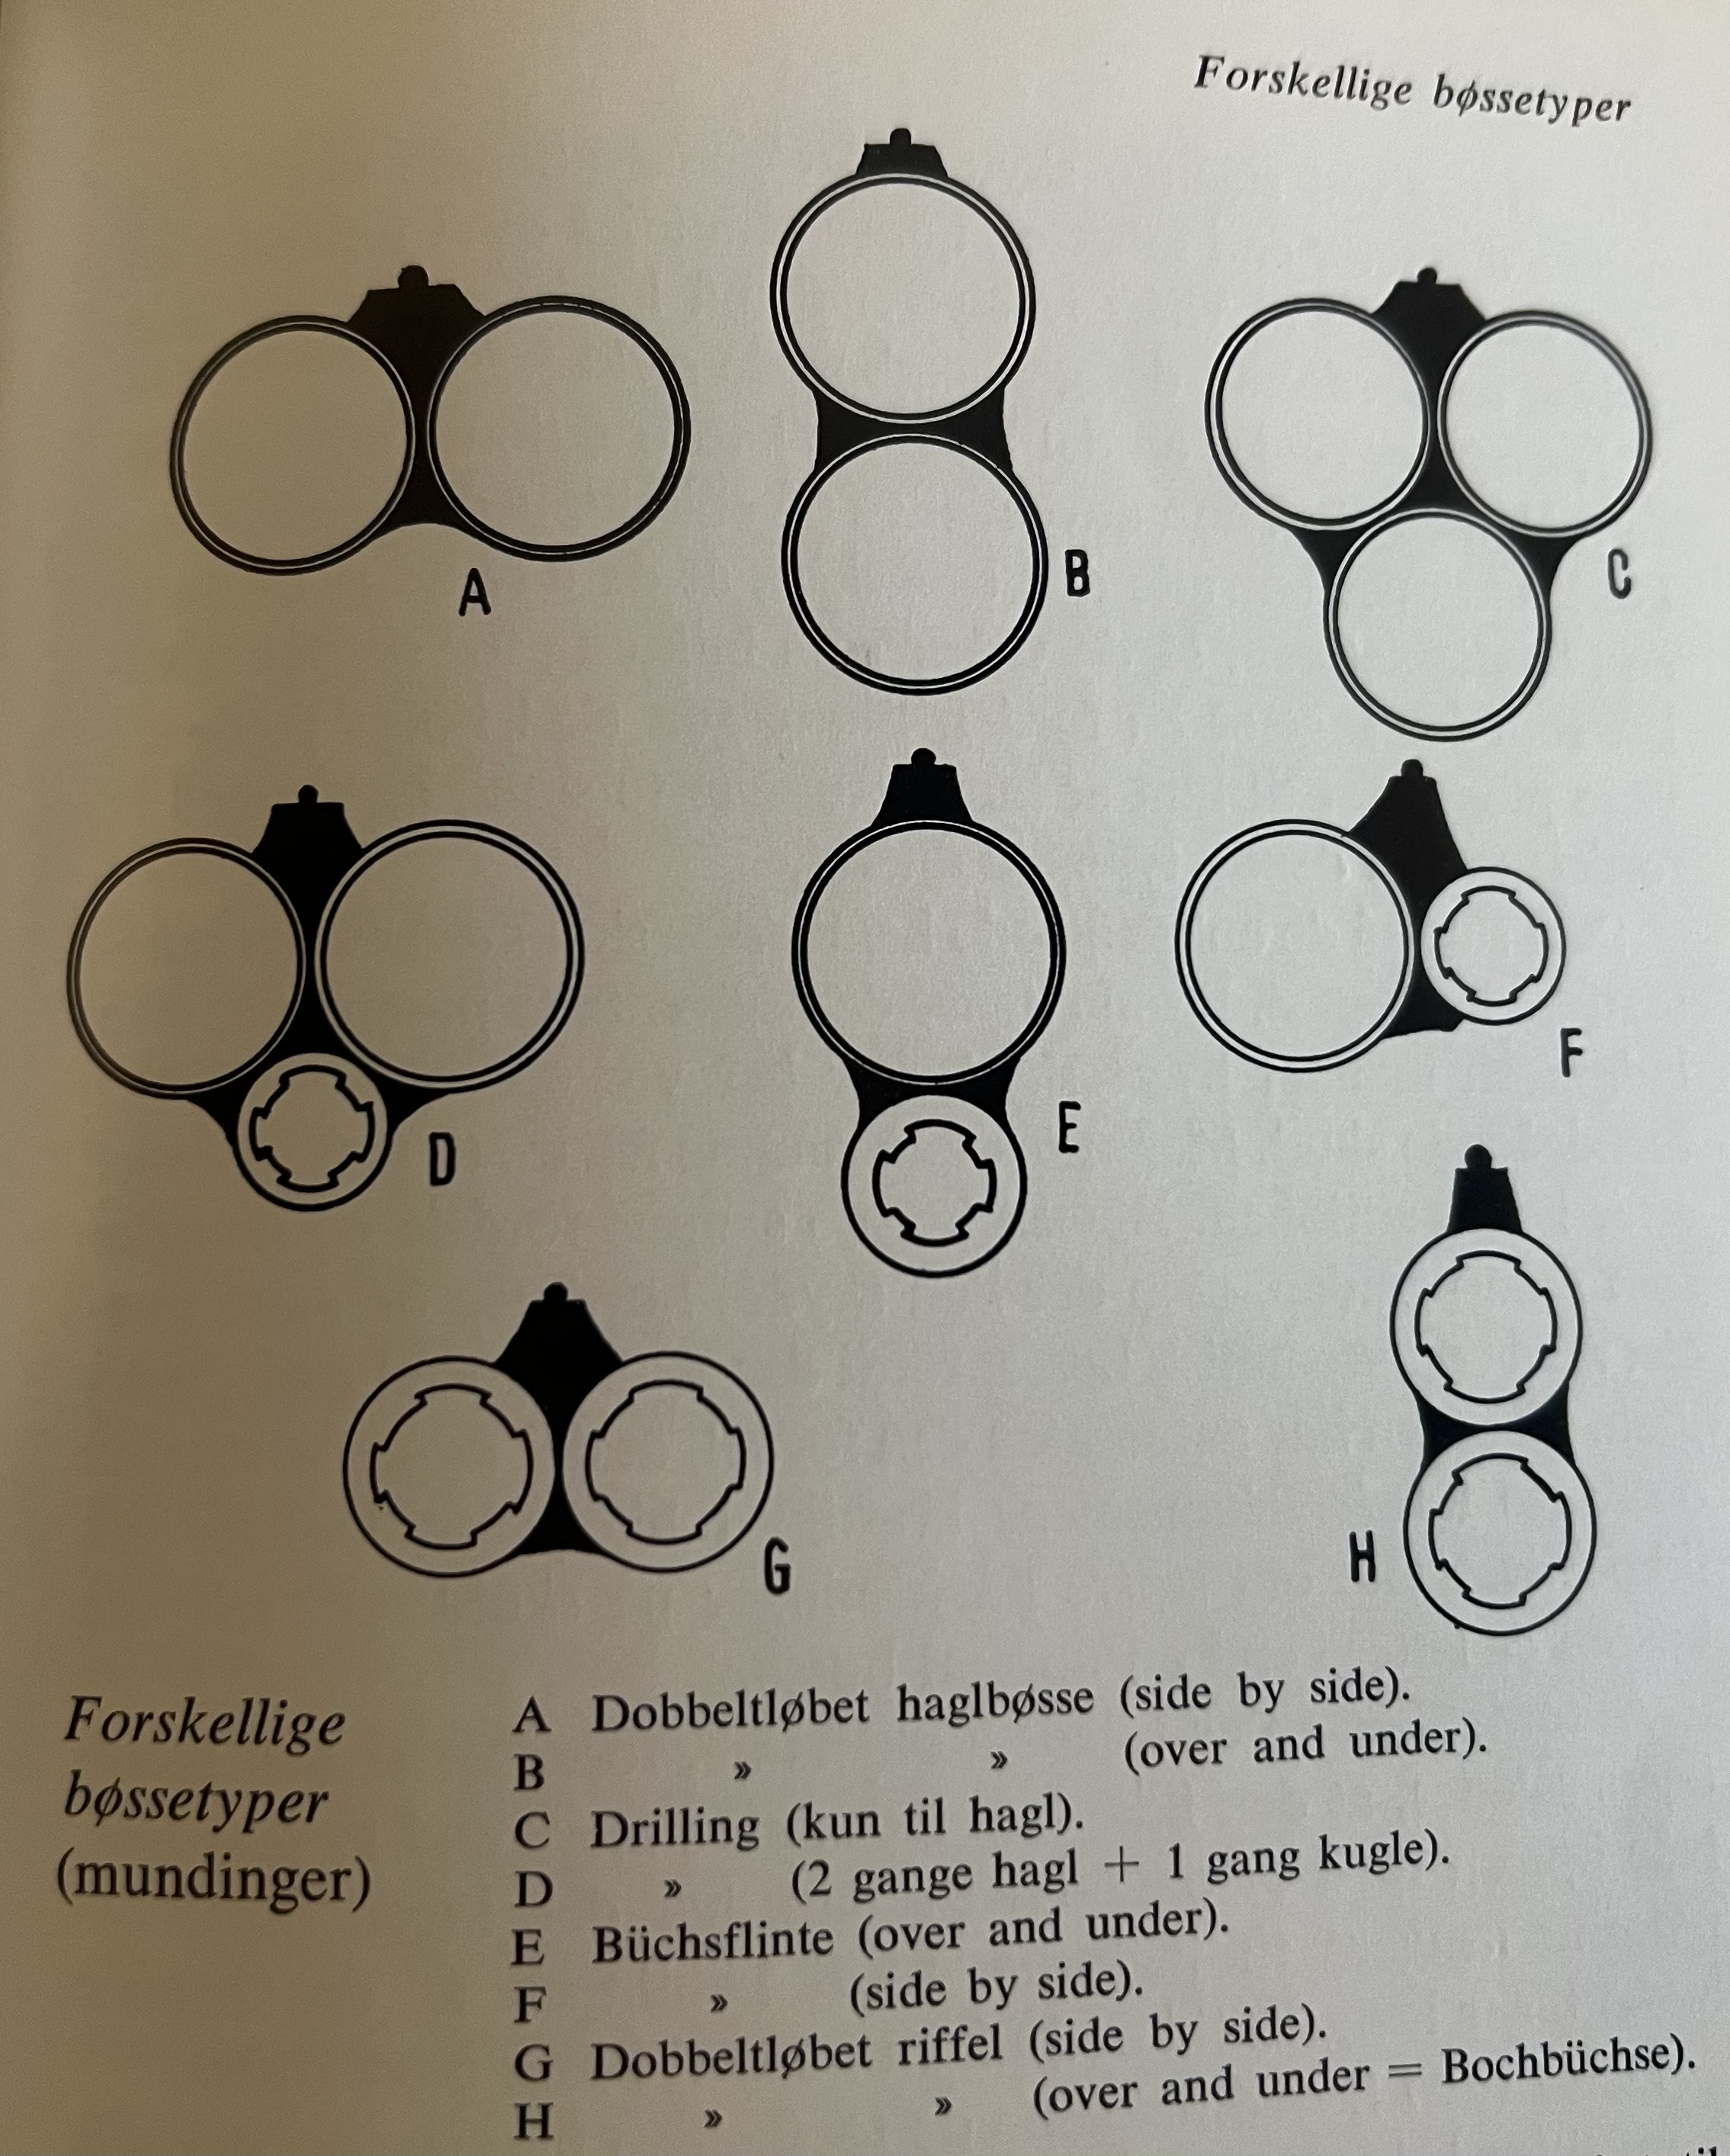
\includegraphics[width=0.3\textwidth]{Billeder/Andet/haglvarianter.jpeg}
        % Eller: [height=0.6\textheight] for højde-baseret skalering
    \end{center}
    
    % Her kan du tilføje tekst under billedet
    \vspace{1em}
    
\end{frame}

\begin{frame}{Haglvåben skæftetyper}
    \begin{center}
        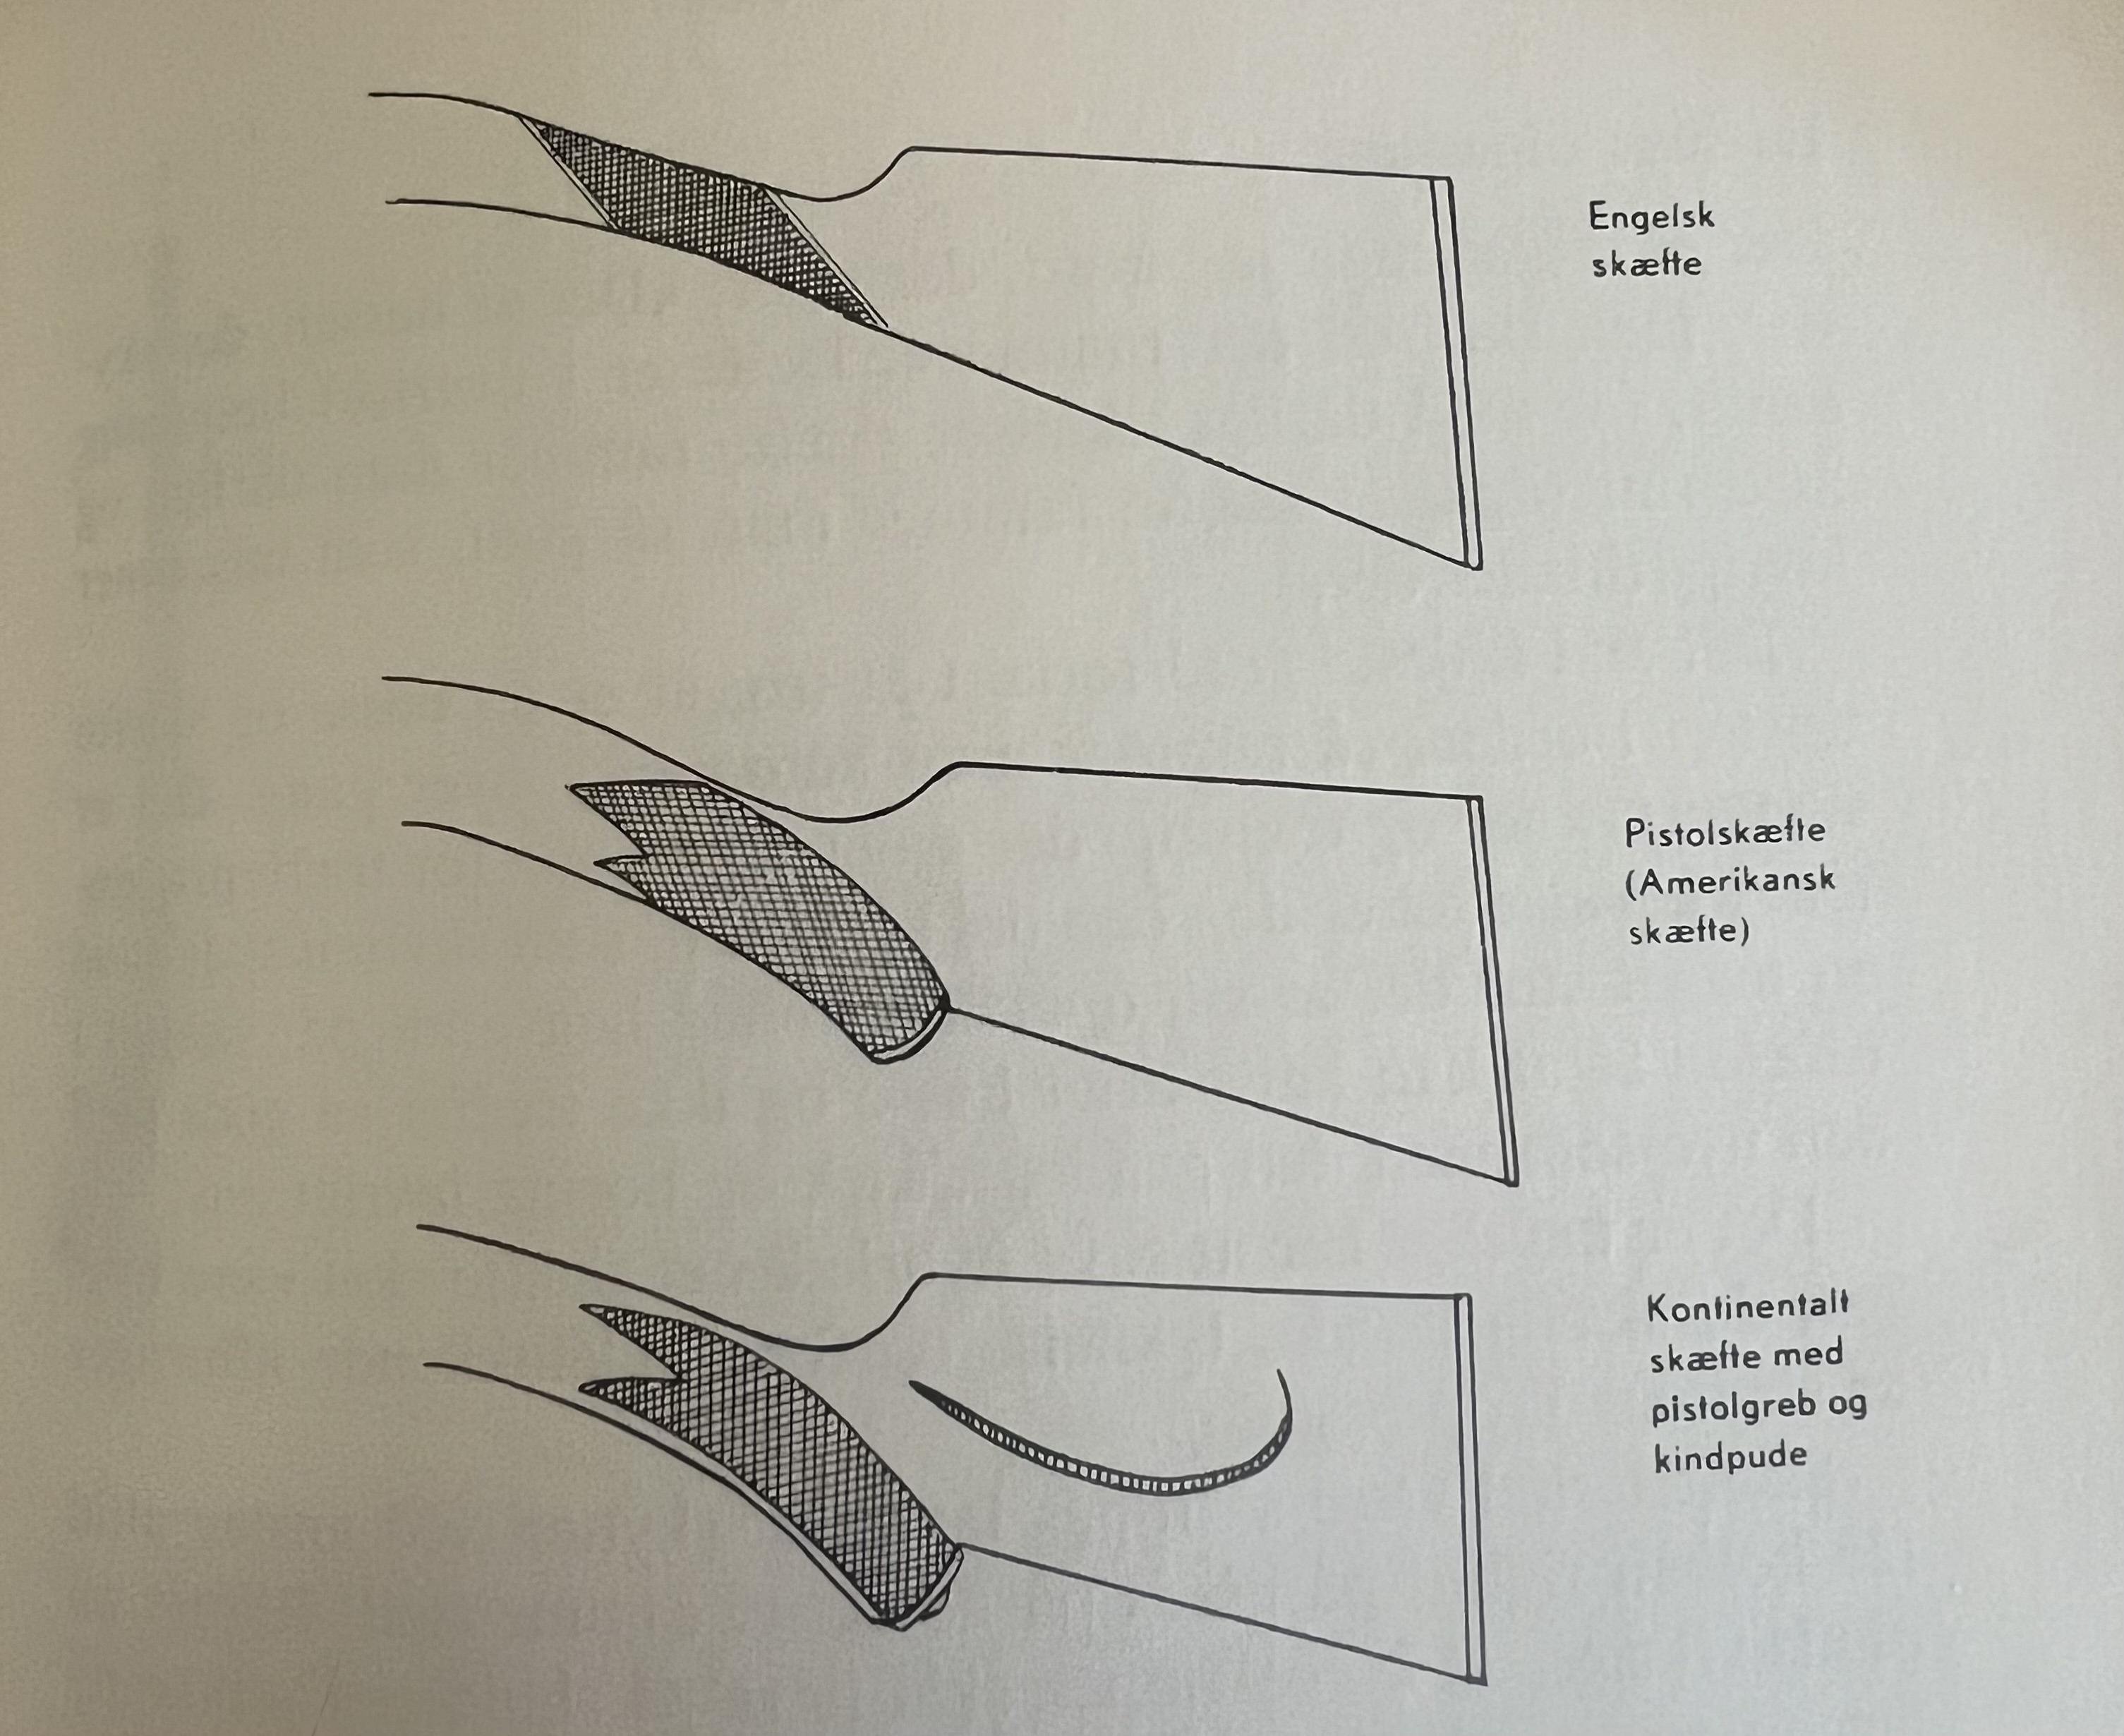
\includegraphics[width=0.5\textwidth]{Billeder/Andet/haglskaefter.jpeg}
        % Eller: [height=0.6\textheight] for højde-baseret skalering
    \end{center}
    
    % Her kan du tilføje tekst under billedet
    \vspace{1em}
    
\end{frame}

\begin{frame}{Haglvåben kalibre}
    \begin{center}
        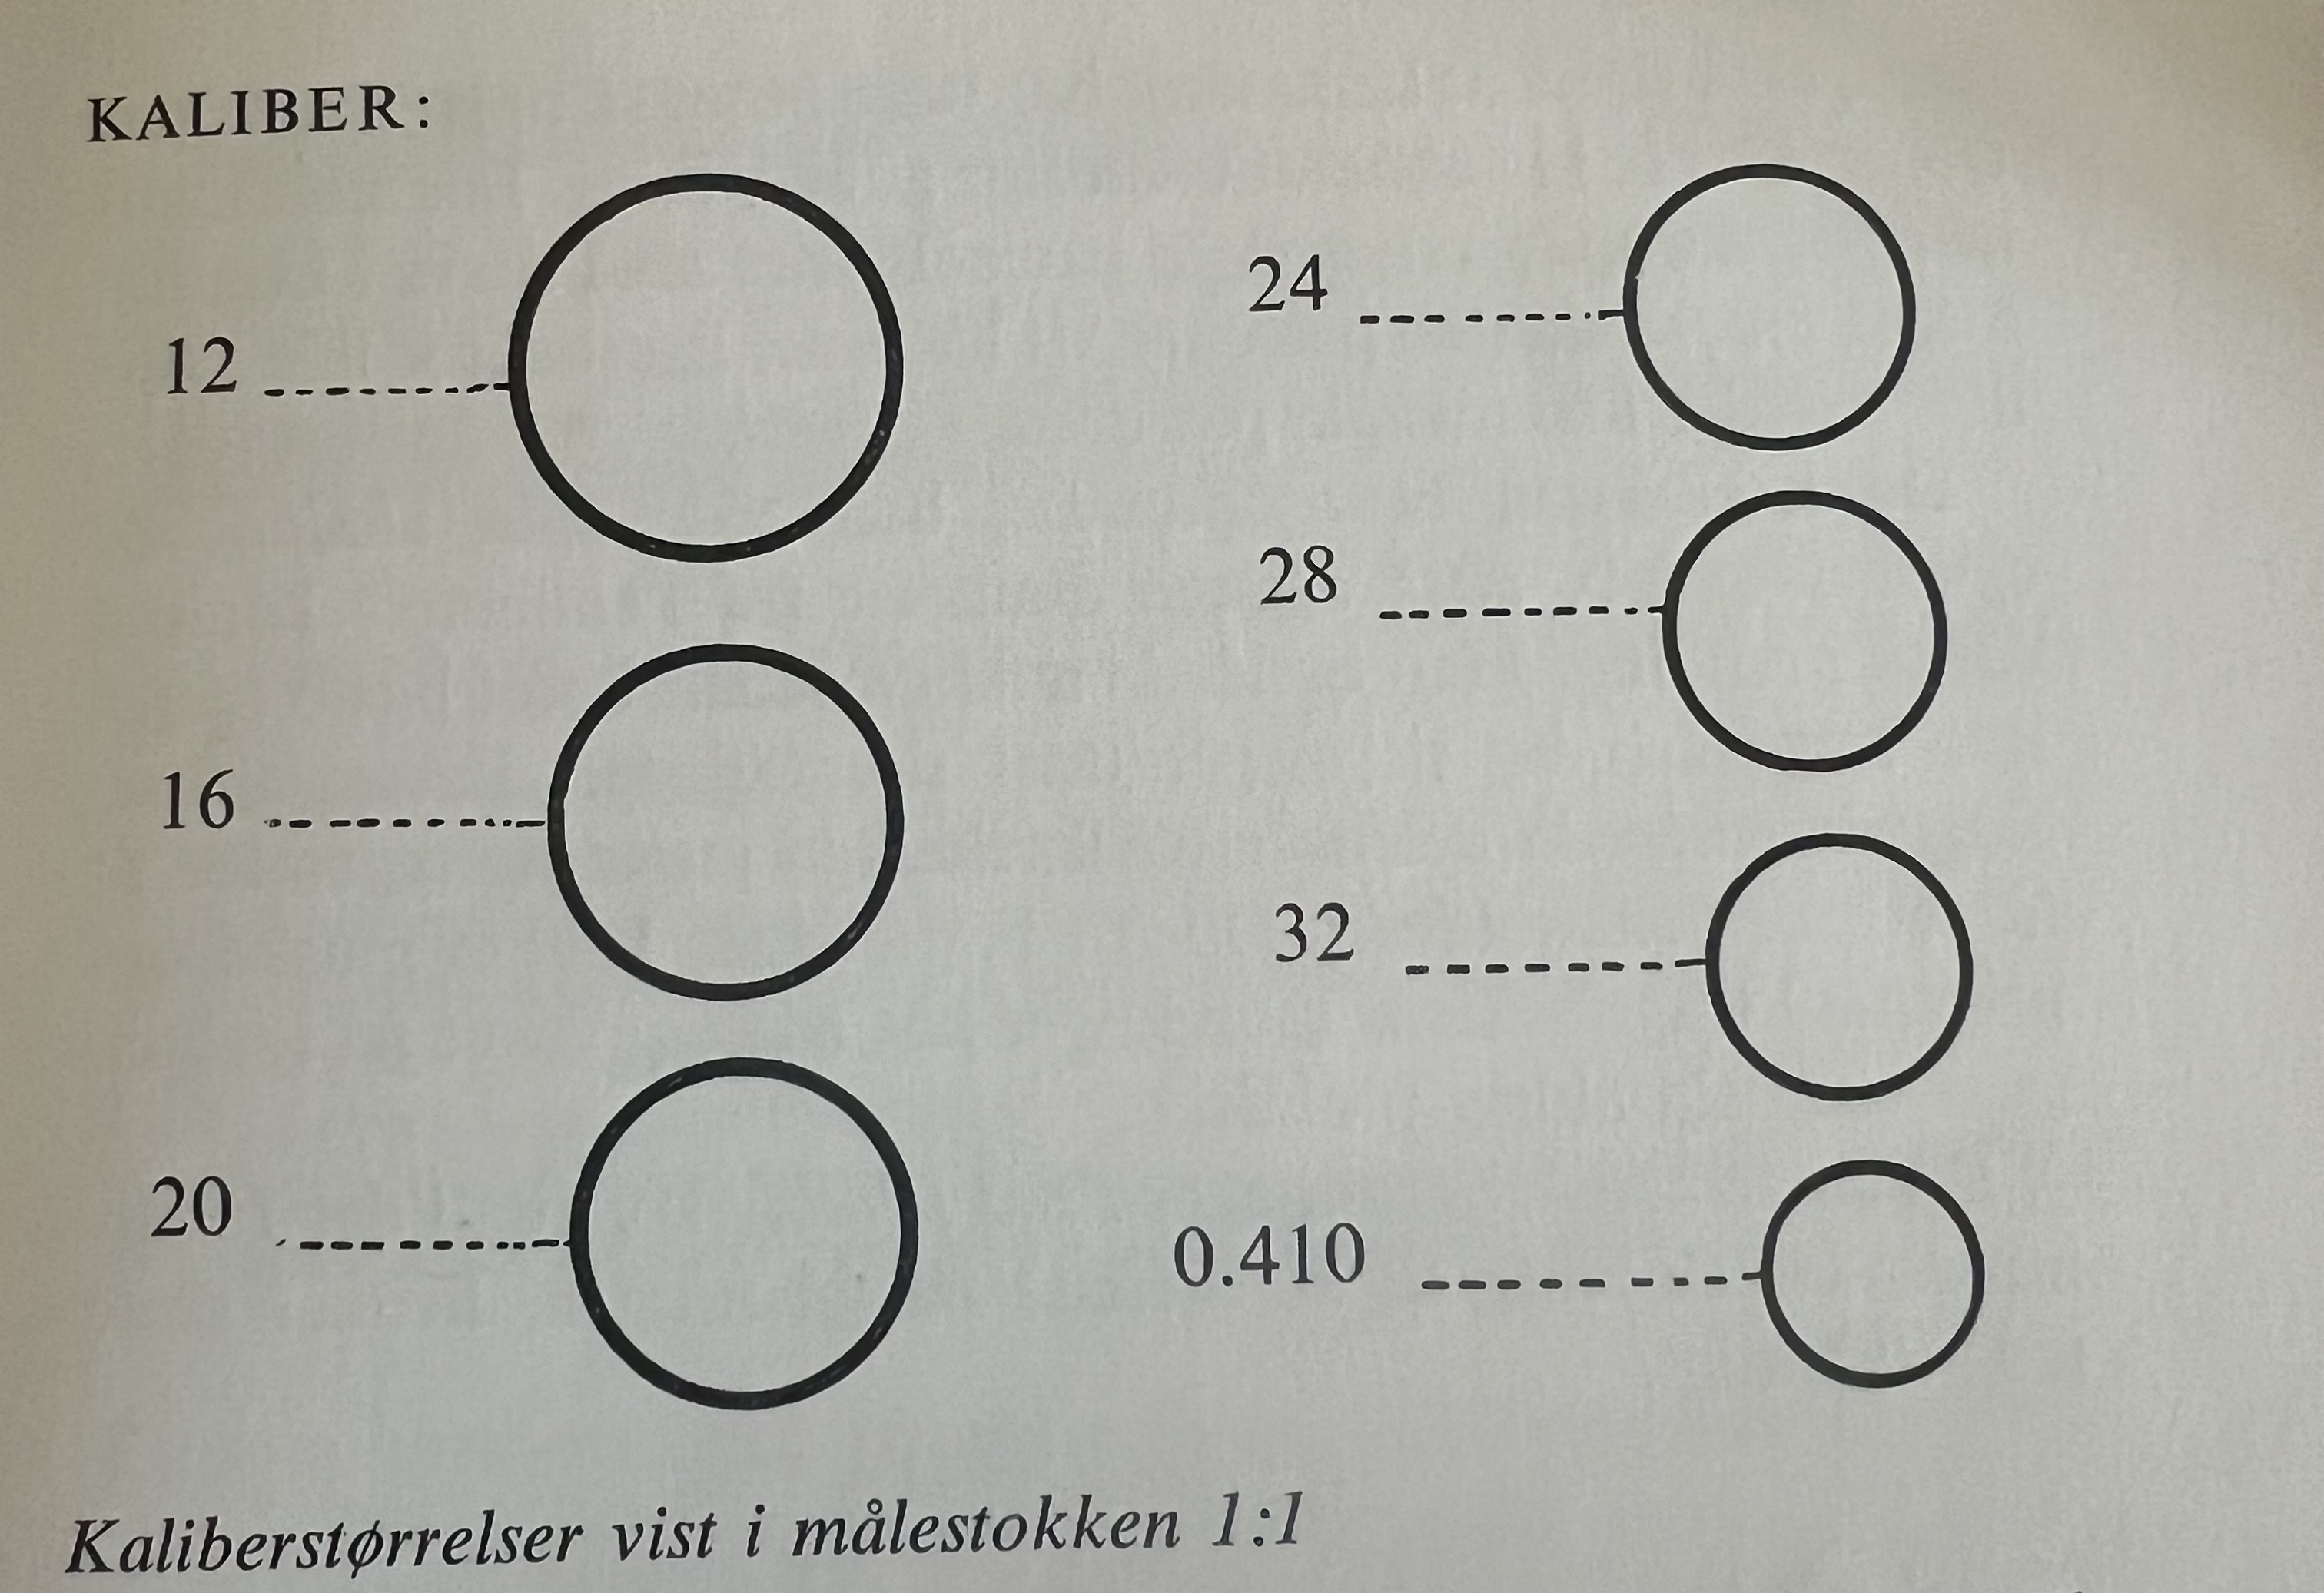
\includegraphics[width=0.5\textwidth]{Billeder/Andet/haglkalibre.jpeg}
        % Eller: [height=0.6\textheight] for højde-baseret skalering
    \end{center}
    
    % Her kan du tilføje tekst under billedet
    \vspace{1em}
    
\end{frame}

\begin{frame}{Sikkerhed med ammunition}
    \begin{itemize}
        \item Forkert kaliber til gevær (tilstopning)
        \item Håndtering af klikker (peg sikker retning, afvrid projektil)
    \end{itemize}
\end{frame}

\begin{frame}{Haglstørrelser og sikkerhedsafstand}
    \begin{center}
        \begin{tabular}{|c|c|c|}
            \hline
            
            \textbf{Nr.} & \textbf{Diameter (mm)} & \textbf{Sikkerhedsafstand (ca. ×100)} \\
            \hline
            Nr. 1 & 4,00 mm & 400 m \\
            Nr. 2 & 3,75 mm & 375 m \\
            Nr. 3 & 3,50 mm & 350 m \\
            Nr. 4 & 3,25 mm & 325 m \\
            Nr. 5 & 3,00 mm & 300 m \\
            Nr. 6 & 2,75 mm & 275 m \\
            Nr. 7 & 2,50 mm & 250 m \\
            \hline
        \end{tabular}
    \end{center}
    
    \vspace{1em}
    \small
    \textbf{Bemærk:} \\
    $\times 100$ er en meget grov tommelfingerregel for potentiel maksimal rækkevidde ved høj affyringsvinkel. \\
    Reelt: Nr. 1–2 hagl kan nå 200–300 m ved flad skud, men op til 400+ m ved stejl vinkel. \\
    Altid hold 200–300 m sikkerhedsafstand til veje, huse, mennesker mv. – uanset haglstørrelse!
\end{frame}

\begin{frame}{Sikkerhedsafstande riffel}
    \begin{itemize}
        \item Alm jagtriffel = 5000 m (5km)
        \item Salonriffel = 3000 m (3km)
    \end{itemize}
\end{frame}